\section{ElasticSearch}
\par Elasticsearch是个开源分布式搜索引擎,它的特点有:分布式,零配置,自动发现,索引自动分片,索引副本机制,Restful风格接口,多数据源,自动搜索负载等。
\par Index names are different indices. Types are just syntactic sugar to add separation between types of documents. If you know Lucene, type is just a field on a doc.目前, Lucene index has Documents and has no notion of types. Types are something added (as best as possible) by elasticsearch. A lucene document is a flat structure(一种扁平结构) key value pair (so objects in json are also translated to this), and a type ends up as another field within the document (called \_type).
\par Then you build a query and in the field (any query that acces a field to execute on), you can specify type1.field1, and in this case, it will be automatically detected, and the query will be wrapped to only be executed match on docs with \_type:type1 (in an efficient manner), on field1. This does mean that across types, having the same field name with different mappings types (for example, type1 has field1 of type numeric, and type2 also has field1 but of type string) should not be done (working on automatically detecting that...).
\par So, the type prefix when you define the field name should allow to only search on a field against that specific type. (At the end of the day, it is wrapped in a filtered query with a \_type:type1 term filter).
\subsection{What's a mapping?}
\par A mapping not only tells ES what is in a field…it tells ES what terms are indexed and searchable.
\par A mapping is composed of one or more ‘analyzers’(相当于Lucene中的Analyzer), which are in turn built with one or more ‘filters’. When ES indexes your document, it passes the field into each specified analyzer, which pass the field to individual filters.
\par Filters are easy to understand: a filter is a function that transforms data. Given a string, it returns another string (after some modifications). A function that converts strings to lowercase is a good example of a filter.
\par An analyzer is simply a group of filters that are executed in-order. So an analyzer may first apply a lowercase filter, then apply a stop-word removal filter(中文分词作为其中一个filter). Once the analyzer is run, the remaining terms are indexed and stored in ES.因此: a mapping is simply a series of instructions on how to transform your input data into searchable, indexed terms.
\par 使用\textbf{curl -XPUT http://localhost:9200/test/item/1 -d '\{"name":"zach", "description": "A Pretty cool guy."\}'}时,ES生成如下的mapping:
\begin{verbatim}
mappings: {
   item: {
      properties: {
         description: { type: string }
         name: { type: string }
      }
   }
}
\end{verbatim}
\par ES猜测到"description"这列的类型为"string",When ES implicitly creates a "string" mapping, it applies the default global analyzer.除非显式地更改analyzer设置,否则ES将使用默认的Standard Analyzer.Standard Analyzer will apply the standard token filter, lowercase filter and stop token filter to your field. 这种情况下,句子末尾的.号和字符'A'将被丢弃.Importantly, even though ES continues to store the original document in it’s original form, the only parts that are searchable are the parts that have been run through an analyzer.So, mappings are not data-types , think of them as instructions on how you will eventually search your data. If you care about stop-words like 'a', you need to change the analyzer so that they aren’t removed.
\subsection{Constructing more complicated mapping}
\par Setting up proper analyzers in ES is all about thinking about the search query. You have to provide instructions to ES about the appropriate transformations so you can search intelligently.
\par The first thing that happens to an input query is tokenization , breaking an input query into smaller chunks called tokens. There are several tokenizers available, which you should explore on your own when you get a chance. The Standard tokenizer is being used in this example, which is a pretty good tokenizer for most English-language search problems. You can query ES to see how it tokenizes a sample sentence:
\begin{verbatim}
curl -X GET "http://localhost:9200/test/_analyze?tokenizer=standard&pretty=true" 
-d 'The quick brown fox is jumping over the lazy dog.'
\end{verbatim}
\par Ok, so our input query has been turned into tokens. Referring back to the mapping, the next step is to apply filters to these tokens. In order, these filters are applied to each token: Standard Token Filter, Lowercase Filter, ASCII Folding Filter.
\begin{verbatim}
curl -X GET "http://localhost:9200/test/_analyze?filter=standard&pretty=true" 
-d 'The quick brown fox is jumping over the lazy dog.'
\end{verbatim}
\par As you can see, we specify both a search and index analyzer. These two separate analyzers instruct ES what to do when it is indexing a field, or searching a field. But why are these needed?
\begin{verbatim}
"partial":{
     "search_analyzer":"full_name",
     "index_analyzer":"partial_name",
     "type":"string"
}
\end{verbatim}
\par The index analyzer is easy to understand. We want to break up our input fields into various tokens so we can later search it. So we instruct ES to use the new partial\_name analyzer that we built, so that it can create nGrams for us.
\par The search analyzer is a little trickier to understand, but crucial to getting good relevance. Imagine querying for “Race”. We want that query to match “race”, “races” and “racecar”. When searching, we want to make sure ES eventually searches with the token “race”. The full\_name analyzer will give us the needed token to search with.
\par If, however, we used the partial\_name nGram analyzer, we would generate a list of nGrams as our search query. The search query “Race” would turn into ["ra", "rac", "race"].Those tokens are then used to search the index. As you might guess, “ra” and “rac” will match a lot of things you don’t want, such as “racket” or “ratify” or “rapport”.
\par So specifying different index and search analyzers is critical when working with things like ngrams. Make sure you always double check what you expect to query ES with…and what is actually being passed to ES.
\subsection{Depth into ElasticSearch}
\par 当使用如下命令搜索时:
\begin{verbatim}
curl -XPOST "http://namenode:9200/_search" -d'
{
    "query": {
      "match_all" : {}
    },
    "filter" : {
      "term" : { "director" : "Francis Ford Coppola"}
    }
}'
\end{verbatim}
没有任何结果,而使用
\begin{verbatim}
curl -XPOST "http://namenode:9200/_search" -d'
{
    "query": {
      "match_all" : {}
    },
    "filter" : {
      "term" : { "year" : "1962"}
    }
}'
\end{verbatim}
\par 却能输出结果,What's going on here?  We've obviously indexed two movies with "Francis Ford Coppola" as director and that's what we see in search results as well. Well, while ES has a JSON object with that data that it returns to us in search results in the form of the \_source property .
\par When we index a document with ElasticSearch it (simplified) does two things: it stores the original data untouched for later retrieval in the form of \_source and it indexes each JSON property into one or more fields in a Lucene index. During the indexing it processes each field according to how the field is mapped. If it isn't mapped , default mappings depending on the fields type (string, number etc) is used.
\par As we haven't supplied any mappings for our index, ElasticSearch uses the default mappings for the director field. This means that in the index the director fields value isn't \textbf{"Francis Ford Coppola"}. Instead it's something like \textbf{["francis", "ford", "coppola"]}. We can verify that by modifying our filter to instead match "francis" (or "ford" or "coppola").
\par So, what to do if we want to filter by the exact name of the director? We modify how it's mapped. There are a number of ways to add mappings to ElasticSearch, through a HTTP request that creates by calling the \_mapping endpoint. Using this approach, we could fix the above issue by adding a mapping for the "director" field , to instruct ElasticSearch not to analyze (tokenize etc.) the field at all.
\begin{verbatim}
curl -X PUT namenode:9200/movies/movie/_mapping -d'
{
   "movie": {
      "properties": {
         "director": {
            "type": "string",
            "index": "not_analyzed"
        }
      }
   }
}'
\end{verbatim}
\par In many cases it's not possible to modify existing mappings. Often the easiest work around for that is to create a new index with the desired mappings and re-index all of the data into the new index. The second problem is that, even if we could add it, we would have limited our ability to search in the director field. That is, while a search for the exact value in the field would match we wouldn't be able to search for single words in the field.
\par 幸运地是存在更简单的办法。We add a mapping that upgrades the field to a multi field. What that means is that we'll map the field multiple times for indexing. Given that one of the ways we map it match the existing mapping both by name and settings that will work fine and we won't have to create a new index.
\begin{verbatim}
curl -XPUT "namenode:9200/movies/movie/_mapping" -d'
{
   "movie": {
      "properties": {
         "director": {
            "type": "multi_field",
            "fields": {
               "director": {"type": "string's"},
               "original": {"type" : "string", "index" : "not_analyzed"}
            }
         }
      }
   }
}'
\end{verbatim}
\subsection{ElasticSearch集群设置}
This will print the number of open files the process can open on startup. Alternatively, you can retrieve the max\_file\_descriptors for each node using the Nodes Info API, with:\\
\textbf{curl -XGET 'namenode:9200/\_nodes/process?pretty=true'},下面是删除ES上名为jdbc的index的Restfule命令:\\
\textbf{curl -XDELETE 'http://namenode:9200/jdbc/'}
\par 配置文件在\textbf{\{\$ES\_HOME\}/config}文件夹下,\textbf{elasticsearch.yml}和\textbf{logging.yml},修改\textbf{elasticsearch.yml}文件中的cluster.name,当集群名称相同时,每个ES节点将会搜索它的伙伴节点,因此必须保证集群内每个节点的cluster.name相同,下面是关闭ES集群的Restful命令:
\begin{verbatim}
# 关闭集群内的某个ES节点'_local'
$ curl -XPOST 'http://namenode:9200/_cluster/nodes/_local/_shutdown'
# 关闭集群内的全部ES节点
$ curl -XPOST 'http://namenode:9200/_shutdown'
\end{verbatim}
\par 注意,如果一台机器上不止一个ES在运行,那么通过\textbf{./bin/elasticsearch}开启的ES的http\_address将会使用9200以上的接口(形如9201,9202,$\cdots$),而相应的transport\_address也递增(形如:9301,9302,$\cdots$),因此,为使用9200端口,可使用上述命令关闭其它ES进程,可通过conf目录下的log文件来查看某些端口是否被占用。\textbf{elasticsearch.yml}文件存在如下配置信息:
\begin{enumerate}[(1)]
\item node.master: true,node.data: true,允许节点存储数据,同时作为主节点;
\item node.master: true,node.data: false,节点不存储数据,但作为集群的协调者;
\item node.master: false,node.data: true,允许节点存储数据,但不作为主节点;
\item node.master: false,node.data: false,节点不存储数据,也不作为协调者,但作为搜索任务的一个承担者;
\item cluster.name: HadoopSearch, node.name: "ES-Slave-02",HadoopSearch必须相同,但node.name每个节点可以自由设置;
\end{enumerate}
如想将ES作为一个服务,需要从github上下载elasticsearch-servicewrapper,然后调用chkconfig,将其添加到/etc/rc[0$\sim$6].d/中。
\begin{verbatim}
curl -L https://github.com/elasticsearch/elasticsearch-servicewrapper/archive/master.zip > master.zip
unzip master.zip
cd elasticsearch-servicewrapper-master/
mv service /opt/elasticsearch/bin
/opt/elasticsearch/bin/service/elasticsearch install
## 如果想卸载该服务调用:
/opt/elasticsearch/bin/service/elasticsearch remove
## 如果想让ES开机启动
chkconfig elasticsearch on  
## 如果想现在开启ES服务
service elasticsearch start 
\end{verbatim}
配置完后,可通过\textsl{curl -X GET 'http://192.168.50.75:9200/\_cluster/nodes?pretty'}命令,查询集群下的节点信息。
\par 为连接hive与ES,运行hive后,在hive命令行内执行\textbf{add jar /opt/elasticsearch-hadoop-1.3.0/dist/elasticsearch-hadoop-1.3.0.jar;}或者hdfs上的jar包:\textbf{add jar hdfs://namenode:9000/elasticsearch-hadoop-1.3.0.jar}可加载elasticsearch-hadoop插件,使用该插件的具体操作如下:
\begin{verbatim}
DROP TABLE IF EXISTS artist_1;
CREATE EXTERNAL TABLE artists_1 (
  cardid STRING, date STRING, time STRING)
STORED BY 'org.elasticsearch.hadoop.hive.ESStorageHandler'
TBLPROPERTIES('es.resource' = 'liubo/artists/',
              'es.host' = '192.168.50.75',
              'es.mapping.names' = 'text:time'
);
-- 集群下应使用'192.168.50.75',而非'localhost'(es-hadoop的默认值)
-- insert data to Elasticsearch from another hive table
INSERT OVERWRITE TABLE artists_1
SELECT * FROM cable.temptable;
\end{verbatim}
\par 下面的代码是将Mysql中的表导入到ES中,建立名为jdbc的index,表名称为jiangsu。
\begin{verbatim}
curl -XPUT 'localhost:9200/_river/jiangsu/_meta' -d '{
    "type" : "jdbc",
    "jdbc" : {
        "driver" : "com.mysql.jdbc.Driver",
        "url" : "jdbc:mysql://192.168.50.75:3306/jsyx",
        "user" : "root",
        "password" : "123456",
        "sql" : "select * from jiangsu"
    },
    "index" : {
        "index" : "jdbc",
        "type" : "jiangsu"
    }
}'
\end{verbatim}
\subsection{ES性能优化}
\par 一个Elasticsearch节点会有多个线程池,但重要的是下面四个:
\begin{itemize}
\item 索引(index):主要是索引数据和删除数据操作(默认是cached类型);
\item 搜索(search):主要是获取,统计和搜索操作(默认是cached类型);
\item 批量操作(bulk):对索引的批量操作,尚且不清楚它是不是原子性的,如果是原子的,则放在MapReduce里是没有问题的;
\item 更新(refresh):主要是更新操作,如当一个文档被索引后,何时能够通过搜索看到该文档;
\end{itemize}
\par 在建立索引(index相当于数据库,type相当于数据库中的表)的过程中,需要修改如下配置参数:
\begin{itemize}
\item index.store.type: mmapfs.因为内存映射文件机制能更好地利用OS缓存;
\item indices.memory.index\_buffer\_size: 30\% 默认值为10\%,表示10\%的内存作为indexing buffer;
\item index.translog.flush\_threshold\_ops: 50000,当写日志数达到50000时,做一次同步;
\item index.refresh\_interval:30s,默认值为1s,新建的索引记录将在1秒钟后查询到;
\end{itemize}
\begin{verbatim}
curl -XPUT 'http://namenode:9200/hivetest/?pretty' -d '{
    "settings" : {
       "index" : {
       "refresh_interval" : "30s",
       "index.store.type": "mmapfs",
       "indices.memory.index_buffer_size": "30%",
       "index.translog.flush_threshold_ops": "50000"
        }
    }
}'
\end{verbatim}
\par 但上述设置性能低下,也不知why?ES索引的过程相对Lucene的索引过程多了分布式数据的扩展,而ES主要是用tranlog进行各节点间的数据平衡,因此设置"index.translog.flush\_threshold\_ops"为"100000",意思是当tranlog数据达到多少条进行一次平衡操作,默认为5000,而这个过程相对而言是比较浪费资源的,必要时可以将这个值设为-1关闭,进而手动进行tranlog平衡。"refresh\_interval"是刷新频率,设置为30s是指索引在生命周期内定时刷新,一但有数据进来就在Lucene里面commit,因此其值设置大些可以提高索引效率。另外,如果有副本存在,数据也会马上同步到副本中去,因此在索引过程中,将副本设为0,待索引完成后将副本个数改回来。
\begin{verbatim}
curl -XPUT 'namenode:9200/hivetest/' #新建一个名为hivetest的索引
curl -XPOST 'namenode:9200/hivetest/_close' #关闭索引,为修改参数做准备
curl -XPUT 'namenode:9200/hivetest/_settings?pretty' -d '{
   "index" : {
      "refresh_interval" : "30s",
      "index.translog.flush_threshold_ops": "100000",
      "number_of_replicas" : 0
   }
}'
curl -XPOST 'namenode:9200/hivetest/_open'
\end{verbatim}
\par Linux主机上硬盘空间有限,经常发现root目录下已没有可利用磁盘空间,为此,将ES的日志和数据输出目录设置在/home目录下,修改config目录下的elasticsearch.yml文件中的选项,其中path.data为索引文件存放目录,path.work为临时文件存放目录,path.logs为日志文件存放目录。
\begin{verbatim}
path.data: /home/elasticSearch/data
path.work: /home/elasticSearch/work
path.logs: /home/elasticSearch/logs
\end{verbatim}
\subsection{Lucene索引}
\subsubsection{Lucene结构}
Lucene基础架构如图\ref{fig-lucene-1}示,
\begin{figure}[htbp]
\centering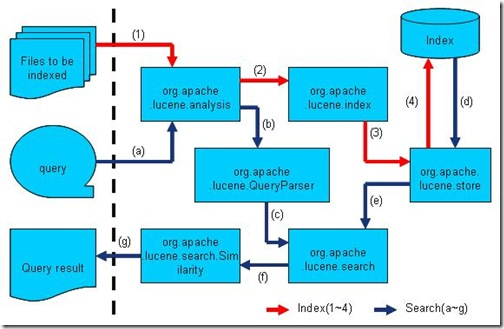
\includegraphics[width=.7\linewidth]{figures/lucene-architect.jpg}
\caption{Lucene基础架构图}\label{fig-lucene-1}
\end{figure} 
\begin{enumerate}[(1)]
\item Lucene的analysis模块主要负责词法分析及语言处理而形成Term。
\item Lucene的index模块主要负责索引的创建,里面有IndexWriter。
\item Lucene的store模块主要负责索引的读写。
\item Lucene的QueryParser主要负责语法分析。
\item Lucene的search模块主要负责对索引的搜索。
\item Lucene的similarity模块主要负责计算相关性。
\end{enumerate}
\par Lucene包含如下几种类型文件:
\begin{description}
\item [.tim]用于存放Term的库,contains the list of terms in each field along with per-term statistics (such as docfreq) and pointers to the frequencies, positions, payload and skip data in the .doc, .pos, and .pay files.
\item [.doc]Frequencies and Skip Data,估计用于计算文档相关性,contains the lists of documents which contain each term, along with the frequency of the term in that document.
\item [.pos]Positions,存储Term位置的文件,contains the lists of positions that each term occurs at within documents,此外,还有.tip类型文件(用于索引Term)和.pay类型文件(做什么,暂时不详)。
\end{description}
\par Lucene包含如下几种jar包:
\begin{enumerate}[(1)]
\item org.apache.lucene.util,一些公用基础设施。
\item org.apache.lucene.analysis,语言分析器,主要用于切分单词(英文根据空格),对中文的扩展支持可改写此类。
\item org.apache.lucene.document,索引存储时的文档结构管理,类似于关系型数据库的关系。
\item org.apache.lucene.index,索引管理,包括索引建立、删除,更新等。
\item org.apache.lucene.queryParser,查询分析器,实现查询关键词间的运算,如与、或、非等,据说写得十分复杂。
\item org.apache.lucene.search,检索管理,根据查询条件,检索得到结果。
\item org.apache.lucene.store,数据存储管理,包括一些底层I/O操作。
\end{enumerate}
\subsubsection{Lucene分词过程}
\par Analyzer类是所有分词器的基类,它是个抽象类,所有的子类必须实现它。它的功能实质上是将输入文本转化为文本特征向量,这里所说的文本特征,可以是词或者是短语,它主要包括四个步骤:(1)分词,将文本解析为单词或短语;(2)归一化,将文本转化为小写;(3)停用词处理,去除一些常用的、无意义的词;(4)提取词干,解决单复数、时态语态等问题。
\par Lucene Analyzer包含两个核心组件,Tokenizer以及TokenFilter。两者的区别在于,前者在字符级别处理流(即前者将字符串转换成Term),而后者则在词语级别处理流(对Term进行转换)。Tokenizer是Analyzer的第一步,其构造函数接收一个Reader(例如BufferedReader)作为参数,而TokenFilter则类似一个拦截器,其参数可以是TokenStream、Tokenizer,甚至是另一个TokenFilter。
\begin{description}
\item [Token]表示文中出现的一个词,它包含了词在文本中的位置信息等等;
\item [Analyzer]将文本转化为TokenStream的工具,Analyzer通过对文本的分析来建立TokenStream;
\item [TokenStream]由一个个Token组成的数据流,可以说Analyzer是一种从文本数据中抽取索引词(Term)的策略。
\item [Tokenizer]处理输入符号流,生成一个个Token;
\item [TokenFilter]处理符号流,输入可以是TokenStream,Tokenizer,TokenFilter;
\end{description}
\par Lucene提供了数十种内置的Tokenizer、TokenFilter以及Analyzer供开发人员使用,事实上大部分时候只需要使用其中几种,比如标准分词器StandardTokenizer、空格分词器WhitespaceTokenizer(按空格分词)、转化为小写格式的LowCaseFilter(将英文单词转换成小写)、提取词干的PoterStemFilter(提取英文词干,比如对英文的过去式,现在进行时等提取词干)以及组合使用StandardTokenizer和多种TokenFilter的StandardAnalyzer。 
\par 处理英文默认的Analyzer为StandardAnalyzer,当处理中文分词和拼音等特殊情况时,需要实现自定义的Analyzer,在处理汉字时最主要的工作是实现一个Tokenizer来分词,TokenFilter(汉字的停用词过滤等)不太复杂,可不做过多考虑。当继承Analyzer时,可override其提供的createComponents方法:
\begin{verbatim}
@Override
protected TokenStreamComponents createComponents(String fieldName,
        final Reader reader) {
    Tokenizer tokenizer = new SoulTokenizer(new BasicAnalysis(reader),
        reader, filter, pstemming);
    return new TokenStreamComponents(tokenizer);
}
\end{verbatim}
\par 上例中的fieldName没有用处,有两个类型的子类TokenFilter和Tokenizer(也可以继承CharTokenizer),Tokenizer通过读取汉字字符串创建词序列List<word>,其中每一word将作为Lucene索引的key,Tokenizer还记录每个word的偏移值,以及在文档中属于第几个word($0,\cdots,n$)等,而TokenFilter则对产生的词序列进行转换(比如过滤等)。 
\subsubsection{TokenStream和AttributeSource}
\par TokenStream是从Document的域(field)中或者查询条件中抽取一个个分词而组成的一个数据流,TokenStream中是一个个的分词(Token),而每个分词又是由一个个的属性(Attribute)组成。对所有的分词来说,每个属性只有一个实例,这些属性都保存在AttributeSource中,而AttributeSource正是TokenStream的父类。
\par TokenStream的工作流程:(1)实例化TokenStream, 添加属性到AttributeSource,或从AttributeSource中获取属性;(2)调用reset()方法,设置stream的初始状态;(3)调用increamStoken()方法,获取下一个分词,这个方法会被docuemnt中的每一个分词调用;(4)调用end()方法来完成一些收尾工作;(5)调用close()方法来释放stream拥有的一些资源。
\par 一个AttributeSource中包含着一个由不同AttributeImpl组成的列表,以及添加和获取它们的一些方法。在同一个AttributeSource实例中,每个属性只有一个单实例。AttributeSource通过AttributeFactory来创建AttributeImpl的实例,通过State来标示每个AttributeImpl的状态。
\begin{verbatim}
private final Map<Class<? extends Attribute>, AttributeImpl> attributes;
private final Map<Class<? extends AttributeImpl>, AttributeImpl> attributeImpls;
\end{verbatim}
\par 上述两个成员保存了两种映射关系,设计这两个映射关系的目的是在该AttributeSource实例中对每个Attribute和AttributeImpl保证只有一个AttributeImpl实例,也就是说,当用具体Attribute或者具体AttributeImpl时,不会每次都新建实例,而是类似于单例设计模式。有如下几种类型的Attribute:
\begin{enumerate}[(1)]
\item CharTermAttributeImpl,保存Token对应的Term文本;
\item FlagsAttributeImpl,在Tokenizer链条中,用以在不同节点间传递标识信息。该类同TypeAttribute有相似的目的,但还是有所不同,Flags可以用于不同TokenFilter之间分词(Token)信息的加密;
\item TypeAttributeImpl,分词的词汇类型,默认值为“word”;
\item KeywordAttributeImpl,用于标识一个分词是否为关键字。TokenStream可以用此属性判断分词(Token)是否为关键字,决定是否进行修改,TokenFilter可以根据分词是否为关键字进行跳过(skip)处理;
\item OffsetAttributeImpl,Token分词的起始字符,结束字符偏移量; 
\item PositionIncrementAttribute,它表示tokenStream中的当前token与前一个token在实际的原文本中相隔的词语数量;
\item PositionLengthAttributeImpl,Token占用的位置个数。
\end{enumerate}
\par 假如原文本:I'm a student. These are apples,生成的TokenSteam:
\begin{verbatim}
[1: I'm]  [2:a]   [3:student]   [4:these]   [5:are ]   [6:apples]
\end{verbatim}
\par 其中PositionIncrementAttribute有点特殊,它表示tokenStream中当前token在实际原文中的位置,比如[2:a]的PositionIncrementAttribute值为1(表示第2个Term)。如果使用停用词表过滤,TokenSteam就变成:[1:I'm],[2:student],[3:apples],此时student的PositionIncrementAttribute值仍然是2,而apples的PositionIncrementAttribute值仍然是5。当搜索短语student apples时,显然用户是要搜索出student和apples紧挨着出现的文档,但由于apples和student的PositionIncrementAttribute值相差很大,说明没有紧挨着。
\subsection{ElasticSearch杂项}
\subsubsection{开发ES插件}
\par 插件一般情况下是一个zip文件,它包含了若干Jar包,为安装插件,依赖于Maven的安装。Maven工程的main目录里应包含三个目录(java,resources,assembly)。新建src/main/resources/es-plugin.properties文件,文件内容为:
\begin{verbatim}
plugin=${project.groupId}.${project.artifactId}
## ${project.groupId}.${project.artifactId}必须与插件类名相同
## 或者直接告诉ES插件类名
plugin=org.soul.elasticSearch.plugin.SoulAnalysisPlugin
\end{verbatim}
\par 然后在配置文件pom.xml的<artifactId>maven-assembly-plugin</artifactId>标签中添加如下内容,为何选中maven-assembly-plugin,这是因为该插件负责打包Maven工程,其中的plugin.xml为打包Project时额外执行的功能:
\begin{verbatim}
<descriptors>
   <descriptor>
    ${basedir}/src/main/assembly/plugin.xml
  </descriptor>
</descriptors>
\end{verbatim}
\par 然后新建src/main/assembly/plugin.xml文件,写入如下语句,告诉Maven对编译生成的classes目录下的所有内容打包,其中的zip表示生成格式为zip,id不具有特别含义。
\begin{verbatim}
<?xml version="1.0"?>
<assembly>
  <id>plugin</id>
  <formats>
     <format>zip</format>
  </formats>
  <fileSets>  
    <fileSet>  
      <directory>${project.build.directory}/classes</directory>
      <outputDirectory>/</outputDirectory>  
    </fileSet>  
  </fileSets>
</assembly>
\end{verbatim}
\par 执行“mvn assembly:single”后,应该生成了zip文件,调用bin/plugin命令,将zip文件注入到ElasticSearch中。
\begin{verbatim}
./bin/plugin  --url file:///home/lau/git/soul_seg/target/releases/soul_seg-0.1.0-plugin.zip  --install soul-analysis
\end{verbatim}
\subsubsection{ES与hive}
\par Hive从0.8.0版本后支持两个虚拟列:\textbf{INPUT\_\_FILE\_\_NAME}(即mapper任务的输出文件名)和\textbf{BLOCK\_\_OFFSET\_\_INSIDE\_\_FILE}(即读取记录在当前文件的全局偏移量)。对于块压缩文件,就是当前块的文件偏移量,即当前块的第一个字节在文件中的偏移量。Simple Example:
\begin{verbatim}
use cable;
select INPUT__FILE__NAME, cardid, BLOCK__OFFSET__INSIDE__FILE from test;
select min(BLOCK__OFFSET__INSIDE__FILE),count(INPUT__FILE__NAME) from test
  where BLOCK__OFFSET__INSIDE__FILE < 12000 group by cardid;
select * from test where BLOCK__OFFSET__INSIDE__FILE < 12000;
\end{verbatim}
\par 开始时将'es.mapping.id' = 'id'写成了'es.mapping.id ' = 'id',由于多了一个空格,程序一直没有获得期望的结果。'es.mapping.id'属性告诉Hive,使用hive1表中的id列的值作为ElasticSearch的\_id域,使用剩余几列的值作为ElasticSearch的\_source。表hive1不是存储在hive内部,所以使用\textbf{EXTERNAL}关键字,对于使用\textbf{EXTERNAL}存储的表,必须提供\textbf{STORED BY}关键字,否则hive无法确定用哪个类来存储外部表。
\par 在向ElasticSearch添加索引过程中,必须提供id域,否则当某MapTask失败若干次时,相同的记录可能会插入很多遍。因为如果不指定id,ES会给当前记录随机分配一个id,这点类似于往数据库中insert记录时,必须保证对相同record,其主键也相同,所以在使用hive向ElasticSearch中插入记录时,其id域为相应行在hdfs文件中的位置。
\begin{verbatim}
set mapred.max.split.size=32000000;
add jar hdfs://namenode:9000/user/liubo/1.jar;
DROP TABLE IF EXISTS hive1;
CREATE EXTERNAL TABLE hive1(
   id STRING,
   cardId STRING, 
   playDate STRING, 
   playTime STRING,
   channel STRING, 
   program STRING
)
STORED BY 'org.elasticsearch.hadoop.hive.ESStorageHandler'
TBLPROPERTIES('es.resource' = 'eshive/hive1/',
              'es.host' = '192.168.50.75',
              'es.mapping.id' = 'id'
);
INSERT OVERWRITE TABLE hive1 SELECT BLOCK__OFFSET__INSIDE__FILE,* FROM testData2;
\end{verbatim}
\subsubsection{ES查询分析}
\par 假如索引中存在词组:[quick] [brown] [fox] [jump] [over] [lazy] [dog]。
\paragraph{Prefix Query}
搜索“qu”时,Prefix Query查询所有前缀为“qu”的Term,因此如果索引中存在“quack”,“quote”和“quarter”等Term,那么查询将匹配到这些Term,查询结果为\textbf{quick OR quack OR quote OR quarter}。如果索引中存在很多类似Term时,查询效率很差。Prefix Query也不能匹配中间字符,如“ball”不能匹配“baseball”,虽然可以采用通配符(Wildcard query)进行功能修正,但伸缩能力十分有限。
\paragraph{N-Grams}
如果输入英文时想匹配到目标串[quick]的任意前缀,应该对[quick]进行转换,其Term序列为:[q]/[qu]/[qui]/[quic]/[quick],这种Analyzer称为Edge NGram。还有一种Analyzer称为N-Grams(字符串P的N-Gram是P中长度为N的所有子串),以“brown”这个单词为例,设置(minGram=1和maxGram=2),N-Grams输出[b]/[r]/[o]/[w]/[n]/[br]/[ro]/[ow]/[wn],而Edge NGram输出[b]/[br](将maxGram设置为5,Edge NGram能输出[b]/[br]/[bro]/[brow]/[brown])。针对document的不同域,应该设置不同的Analyzer,在英文网页中,一般只对标题和关键词建立NGrams索引。下面定义了名为autocomplete的\textbf{Analyzer},然后通过\textbf{multi\_field}关键字添加了额外的autocomplete分析器。
\begin{verbatim}
{
  "settings":{
    "analysis":{
      "analyzer":{
        "autocomplete":{
          "type":"custom",
          "tokenizer":"standard",
          "filter":[ "standard", "lowercase", "stop", "kstem", "ngram" ] 
        }
      }
    }
  }
}
{
  "articles":{
    "properties":{
      "name":{
        "type":"multi_field",
        "fields":{
          "name":{
            "type":"string"
          },
          "autocomplete":{
            "analyzer":"autocomplete",
            "type":"string"
          }
        }
      }
    }
  }
}
\end{verbatim}
\par 搜索时可使用name来访问name域的默认版本,或者使用name.autocomplete访问另外一个版本。
\subsection{ElasticSearch源码分析}
\par elasticSearch对Google Guice进行了简单的封装,通过ModulesBuilder类构建es的模块,一个es节点包括下面模块:
\begin{multicols}{2}
\begin{itemize}
\item PluginsModule:插件模块
\item SettingsModule:参数设置模块
\item NodeModule:节点管理模块
\item NetworkModule:网络管理模块
\item NodeCacheModule:分布式缓存模块
\item ScriptModule:脚本处理模块
\item JmxModule:Java管理扩展模块
\item EnvironmentModule:环境模块
\item NodeEnvironmentModule:节点环境模块
\item ClusterNameModule:集群名模块
\item ThreadPoolModule:线程池模块
\item DiscoveryModule:节点自动发现模块
\item ClusterModule:集群模块
\item RestModule:rest模块
\item TransportModule:tcp模块
\item HttpServerModule:http模块
\item RiversModule:river模块
\item IndicesModule:索引模块
\item SearchModule:搜索模块
\item ActionModule:行为模块
\item MonitorModule:监控模块
\item GatewayModule:持久化模块
\item NodeClientModule:客户端模块
\end{itemize}
\end{multicols}
\begin{enumerate}[(1)]
\item 有"/\_analyze"和"/\{index\}/\_analyze两种,接受GET和POST方法,在org/elasticsearch/rest/action/admin/indices/analyze/RestAnalyzeAction.java中被处理;在ActionModule中,存在一个注册函数registerAction(AnalyzeAction.INSTANCE, TransportAnalyzeAction.class),因此请求将由TransportAnalyzeAction类处理。
\item "/\{index\}/\_close",只接受POST方法,在org/elasticsearch/rest/action/admin/indices/close/RestCloseIndexAction.java中被处理;
\item  创建一个新的索引,json参数中包括settings和mappings(\textbf{注意并非endpoint中的\_mapping}),只有"/\{index\}"一种操作,接受POST和PUT两种方法,在org/elasticsearch/rest/action/admin/indices/create/RestCreateIndexAction.java中处理;
\item rest.action目录负责接受,解释Rest请求。client.node负责管理节点客户端请求。action.admin.indices目录负责处理Rest请求中的动作。
\end{enumerate}
